\documentclass[conference]{IEEEtran}
\IEEEoverridecommandlockouts
% The preceding line is only needed to identify funding in the first footnote. If that is unneeded, please comment it out.
\usepackage{cite}
\usepackage{amsmath,amssymb,amsfonts}
\usepackage{algorithmic}
\usepackage{graphicx}
\usepackage{textcomp}
\usepackage{xcolor}
\usepackage[utf8]{inputenc}
\def\BibTeX{{\rm B\kern-.05em{\sc i\kern-.025em b}\kern-.08em
    T\kern-.1667em\lower.7ex\hbox{E}\kern-.125emX}}
\begin{document}

\title{Towards community and expert detection on open source global development}

\author{\IEEEauthorblockN{Vinicius Schettino}
\IEEEauthorblockA{\textit{Computer Science Postgraduate Program}\\
\textit{Federal University of Juiz de Fora}\\
Juiz de Fora, Brazil \\
vinicius.schettino@ice.ufjf.br}
\and
\IEEEauthorblockN{Vitor Horta}
\IEEEauthorblockA{\textit{Computer Science Postgraduate Program}\\
\textit{Federal University of Juiz de Fora}\\
Juiz de Fora, Brazil \\
vitor.horta@ice.ufjf.br}
\and
\IEEEauthorblockN{Marco Antônio P. Araújo}
\IEEEauthorblockA{\textit{Computer Science Postgraduate Program}\\
\textit{Federal University of Juiz de Fora}\\
Juiz de Fora, Brazil \\
marco.araujo@ufjf.edu.br}
\and
\IEEEauthorblockN{Victor Ströele}
\IEEEauthorblockA{\textit{Computer Science Postgraduate Program}\\
\textit{Federal University of Juiz de Fora}\\
Juiz de Fora, Brazil \\
victor.stroele@ufjf.edu.br}
}

\maketitle

\begin{abstract}
This document is a model and instructions for \LaTeX.
This and the IEEEtran.cls file define the components of your paper [title, text, heads, etc.]. *CRITICAL: Do Not Use Symbols, Special Characters, Footnotes,
or Math in Paper Title or Abstract.
\end{abstract}

\begin{IEEEkeywords}
component, formatting, style, styling, insert
\end{IEEEkeywords}

\section{Introduction}
Global software development motivates automatic approaches to find experts to aid in critical tasks. Large amount of technical data available is hard to gather and use to manually find suitable human resources to help, specially for newcommers.

Those experts are developers with core importance to software projects. They can be helpful in different tasks, such as question routing \cite{sun2018}, code review \cite{xia2017} and bug fixing \cite{cavalcanti2014}. Their expertise often perpasses technical knowledge or experience in a given technology, such as progamming language. More than that, there is value to identify people as suitable source of help and information on software design, modules, development process and other project specific activities.

Finding those experts is harder on global software development. Distributed teams, different  cultures, levels of knowledge, dedication and goals increases traditional collaboration threats \cite{casey2010}. This scenario unveils the urge of automated tools to ease finding suitable partners to specific tasks. A similar issue concern open source development, that have collaboration and a active community on its very foundation \cite{gutwin2004}. Specially for newcomers, who might have a hard time finding help (in the context of question/answering) or someone to approve his changeset (in the context of code review), find suitable developers to aid can ease the path they will endure. Also, a bad initial experience on a begginer's first interaction with the community can discourage future contributions \cite{Bosu2014}.

GitHub is becoming one of the most important source of software artifacts, home for millions of open source projects and host of global software development workflows. Many studies use GitHub's data specially because of its size and features such as RESTful API, that contributes to data integration~\cite{kalliamvakou2014}. Today, more than 67 million (25 million active) projects and 24 millions users are hosted on GitHub\footnote{https://octoverse.github.com/}.

GitHub workflow is based on issues and pullrequests. Issues represent feature/support requests and bug reporting that are organized by predefined labels. Contributors open pull requests in order to merge a code change up to the main codebase. In this moment, project core members evaluate the contribution, asserting that the change follows guidelines and overall goals of the project. This model is called pull based method \cite{gousios2014}.

Since projects hosted on GitHub can reach thousands of contributors and dozens of core members distributed around de globe, find suitable people to help or review can turn into a challenge. Beyond technical expertise, collaborative work demands other skills and aspects in order to be efficient. For instance, worktime, timezone and language proficiency can shatter collaboration quality \cite{rubin2016}. However, those who have interacted before have less chance of facing those problems. Thus, finding experts that have already proven themselves as suitable contributors in previous interactions may help those in need of aid~\cite{aggarwal2011}.

Therefore, this paper's goal is to find experts whitin open source projects that can be helpful to community members. We seek not only to find technical expertise, but also collaborative capacity, that can be translated as time for helping, project workflow and design knowledge, helping expertise and a history of previous interactions.

To support this goal, we propose a collaborative network using pullrequest data from a GitHub's project. The network design aims to bring forth expert developers through a clusterization process. We hipotetisize that cores of the detected clusters are important figures whitin the cluster as a collaboration partner. We propose the use of NetSCAN~\cite{horta2018}, an overlapping community detection algorithm.

\section{Related Work}

Detecting influential nodes in social networks is a broader problem with significance in several contexts, such as false news propagation\cite{johansson2017}. There are different methods that, in order to find those individuals, use community detection algorithms and graph-related metrics \cite{jalayer2018, simsek2018}. However, they are not validated on software networks nor take collaboration information on their approaches.

There are previous contributions to this field of research, where the main goal is to find experts with software repository data. Many proposed finding suitable code reviewers based on their technical and review expertise \cite{yu2014,xia2017}, although collaboration based approaches \cite{ouni2016,zanjani2016} are relatively new, thus still under explored.

There are also authors that explored mining software repositories to find experts, with focus on collaboration \cite{mo2015}. The main idea is to use social and programming behaviors to point out experts, using a collaborative network and multi-source PageRank algorithm \cite{page1998}. However, they did not use pullrequest data and others datasources from GitHub workflow, also limitating the expertise skills to progamming languages, excluding other technical and process aspects idiosyncratic of each project. Those are gaps we intend to fill with this research.

In summary, there are three aspects that together make our proposal different from previous approaches:

\begin{itemize}
  \item We present a collaboration driven and project based method for finding experts within certain groups.
  \item The highlighted individuals can be expert in project workflow/design specific topics, such as ``\textit{performance}'' or ``\textit{documentation}'', not limited to progamming language or other research narrowed domain.
  \item Our collaboration network is designed over the pull based method \cite{gousios2014}, focusing on solving problems of this workflow and global software development.
\end{itemize}

\section{Collaborative Network Model}

Social networks can be represented as sets of nodes connected by edges. This approach seek to reflect relantionships between individuals and the way they interact. There are different lights and grains this data can be analysed, depending on which conclusions the observer want to draw.

Software development social networks represent developers and their interactions on the development process, such as coding, review, discussion and knowledge exchange. GitHub's provide these informations throught a RESTful API\footnote{https://developer.github.com/v3/}, allowing third part developers to dump a given project's data programmatically. The data needed pass through a consolidation process and is loaded to a neo4j instance, a graph oriented database designed to perform well on graph operations and support a better model understanding.

The nodes are developers, and edges are directed relationships of pullrequests revisions. When a developer creates a review comment on a pull request, it creates edge that goes from the commenter to the pullrequest author. Therefore, the model is a bidirectional graph $ G = (V, E) $ where $ V ={v_0, v_1, ... , v_n} $ represent the set of $n$ developers and $E$ is the set of triples (edges) $e_i_j = (v_i, v_j, w)$ between individuals $v_i$ and $v_j$. The weight $w$ is formulated to show how developers influence each other. It represents the contribution share someone have over the colleague. To avoid detecting experts that were influential in the past but are away from the project now, with their collaboration capacity arguabilly decreased, older interactions worth less to the weight count~\eqref{eq:penalization}}. Each interaction $k$ (represented by $inter(v_i,v_j, k)$) between developers $v_i$ and $v_j$ value decreases exponentially the older it gets. The total penalized value is the sum of all interaction values between two given developers.
With the penalized aggregate value, the weight $w_i_j$ can be calculated~\eqref{eq:weight}}}. $W(v_i,v_j)$ represents how much of $v_j$ interaction came from $v_i$. Thus, $w_i_j$ is always comprised between (0,1]. The closer $w_i_j$ is from 1, greater is the influence of $v_i$ over $v_j$. Also, $w_i_j = 1$ means $v_i$ is responsible for all interaction $v_j$ received.



\begin{equation}
P(v_i,v_j)=\sum\limits_{k=1}^{n}\frac{1}{\exp{days(inter(v_i,v_j, k))}}\label{eq:penalization}
\end{equation}

\begin{equation}
W(v_i,v_j)=\frac{P(v_i,v_j)}{\sum\limits_{k=1}^{n}{P(v_j,v_k)}}\label{eq:weight}
\end{equation}


Influential nodes tends to have many relationships and high participation on interactions. However, relationships between two influential nodes tend to have lower weights, since they interact with many individuals. Casual contributors tend to concentrate their relationships on influential proactive developers, giving them higher weights on these cases. Habitual contributors (including core members) tend to interact with good collaborators often, giving them higher weights as well. Fig.~\ref{fig:graph} shows the graphical representation of how two developers might be connected on the proposed model.

\begin{figure}[htbp]
\centerline{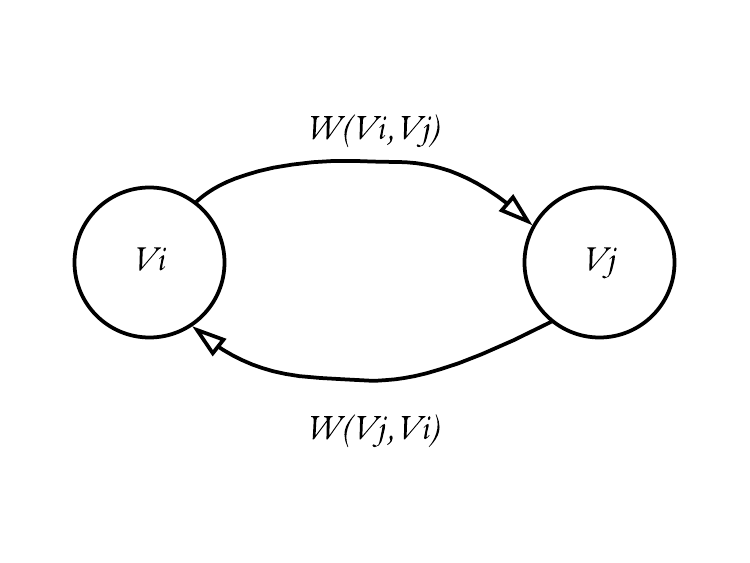
\includegraphics{graph}}
\caption{Graphical representation of developer's relations.}
\label{fig:graph}
\end{figure}

\subsection{Network Topology}

\subsection{Results}

\subsection{Future Work}

\subsection{Conclusions}

Number equations consecutively. To make your
equations more compact, you may use the solidus (~/~), the exp function, or
appropriate exponents. Italicize Roman symbols for quantities and variables,
but not Greek symbols. Use a long dash rather than a hyphen for a minus
sign. Punctuate equations with commas or periods when they are part of a
sentence, as in:
\begin{equation}
a+b=\gamma\label{eq}
\end{equation}

Be sure that the
symbols in your equation have been defined before or immediately following
the equation. Use ``\eqref{eq}'', not ``Eq.~\eqref{eq}'' or ``equation \eqref{eq}'', except at
the beginning of a sentence: ``Equation \eqref{eq} is . . .''

\subsection{\LaTeX-Specific Advice}

Please use ``soft'' (e.g., \verb|\eqref{Eq}|) cross references instead
of ``hard'' references (e.g., \verb|(1)|). That will make it possible
to combine sections, add equations, or change the order of figures or
citations without having to go through the file line by line.

Please don't use the \verb|{eqnarray}| equation environment. Use
\verb|{align}| or \verb|{IEEEeqnarray}| instead. The \verb|{eqnarray}|
environment leaves unsightly spaces around relation symbols.

Please note that the \verb|{subequations}| environment in {\LaTeX}
will increment the main equation counter even when there are no
equation numbers displayed. If you forget that, you might write an
article in which the equation numbers skip from (17) to (20), causing
the copy editors to wonder if you've discovered a new method of
counting.

{\BibTeX} does not work by magic. It doesn't get the bibliographic
data from thin air but from .bib files. If you use {\BibTeX} to produce a
bibliography you must send the .bib files.

{\LaTeX} can't read your mind. If you assign the same label to a
subsubsection and a table, you might find that Table I has been cross
referenced as Table IV-B3.

{\LaTeX} does not have precognitive abilities. If you put a
\verb|\label| command before the command that updates the counter it's
supposed to be using, the label will pick up the last counter to be
cross referenced instead. In particular, a \verb|\label| command
should not go before the caption of a figure or a table.

Do not use \verb|\nonumber| inside the \verb|{array}| environment. It
will not stop equation numbers inside \verb|{array}| (there won't be
any anyway) and it might stop a wanted equation number in the
surrounding equation.

\subsection{Some Common Mistakes}\label{SCM}
\begin{itemize}
\item The word ``data'' is plural, not singular.
\item The subscript for the permeability of vacuum $\mu_{0}$, and other common scientific constants, is zero with subscript formatting, not a lowercase letter ``o''.
\item In American English, commas, semicolons, periods, question and exclamation marks are located within quotation marks only when a complete thought or name is cited, such as a title or full quotation. When quotation marks are used, instead of a bold or italic typeface, to highlight a word or phrase, punctuation should appear outside of the quotation marks. A parenthetical phrase or statement at the end of a sentence is punctuated outside of the closing parenthesis (like this). (A parenthetical sentence is punctuated within the parentheses.)
\item A graph within a graph is an ``inset'', not an ``insert''. The word alternatively is preferred to the word ``alternately'' (unless you really mean something that alternates).
\item Do not use the word ``essentially'' to mean ``approximately'' or ``effectively''.
\item In your paper title, if the words ``that uses'' can accurately replace the word ``using'', capitalize the ``u''; if not, keep using lower-cased.
\item Be aware of the different meanings of the homophones ``affect'' and ``effect'', ``complement'' and ``compliment'', ``discreet'' and ``discrete'', ``principal'' and ``principle''.
\item Do not confuse ``imply'' and ``infer''.
\item The prefix ``non'' is not a word; it should be joined to the word it modifies, usually without a hyphen.
\item There is no period after the ``et'' in the Latin abbreviation ``et al.''.
\item The abbreviation ``i.e.'' means ``that is'', and the abbreviation ``e.g.'' means ``for example''.
\end{itemize}

\subsection{Authors and Affiliations}
\textbf{The class file is designed for, but not limited to, six authors.} A
minimum of one author is required for all conference articles. Author names
should be listed starting from left to right and then moving down to the
next line. This is the author sequence that will be used in future citations
and by indexing services. Names should not be listed in columns nor group by
affiliation. Please keep your affiliations as succinct as possible (for
example, do not differentiate among departments of the same organization).

\subsection{Identify the Headings}
Headings, or heads, are organizational devices that guide the reader through
your paper. There are two types: component heads and text heads.

Component heads identify the different components of your paper and are not
topically subordinate to each other. Examples include Acknowledgments and
References and, for these, the correct style to use is ``Heading 5''. Use
``figure caption'' for your Figure captions, and ``table head'' for your
table title. Run-in heads, such as ``Abstract'', will require you to apply a
style (in this case, italic) in addition to the style provided by the drop
down menu to differentiate the head from the text.

Text heads organize the topics on a relational, hierarchical basis. For
example, the paper title is the primary text head because all subsequent
material relates and elaborates on this one topic. If there are two or more
sub-topics, the next level head (uppercase Roman numerals) should be used
and, conversely, if there are not at least two sub-topics, then no subheads
should be introduced.

\subsection{Figures and Tables}
\paragraph{Positioning Figures and Tables} Place figures and tables at the top and
bottom of columns. Avoid placing them in the middle of columns. Large
figures and tables may span across both columns. Figure captions should be
below the figures; table heads should appear above the tables. Insert
figures and tables after they are cited in the text. Use the abbreviation
``Fig.~\ref{fig}'', even at the beginning of a sentence.

\begin{table}[htbp]
\caption{Table Type Styles}
\begin{center}
\begin{tabular}{|c|c|c|c|}
\hline
\textbf{Table}&\multicolumn{3}{|c|}{\textbf{Table Column Head}} \\
\cline{2-4}
\textbf{Head} & \textbf{\textit{Table column subhead}}& \textbf{\textit{Subhead}}& \textbf{\textit{Subhead}} \\
\hline
copy& More table copy$^{\mathrm{a}}$& &  \\
\hline
\multicolumn{4}{l}{$^{\mathrm{a}}$Sample of a Table footnote.}
\end{tabular}
\label{tab1}
\end{center}
\end{table}

\begin{figure}[htbp]
\centerline{\includegraphics{fig1.png}}
\caption{Example of a figure caption.}
\label{fig}
\end{figure}

Figure Labels: Use 8 point Times New Roman for Figure labels. Use words
rather than symbols or abbreviations when writing Figure axis labels to
avoid confusing the reader. As an example, write the quantity
``Magnetization'', or ``Magnetization, M'', not just ``M''. If including
units in the label, present them within parentheses. Do not label axes only
with units. In the example, write ``Magnetization (A/m)'' or ``Magnetization
\{A[m(1)]\}'', not just ``A/m''. Do not label axes with a ratio of
quantities and units. For example, write ``Temperature (K)'', not
``Temperature/K''.

\section*{Acknowledgment}

The preferred spelling of the word ``acknowledgment'' in America is without
an ``e'' after the ``g''. Avoid the stilted expression ``one of us (R. B.
G.) thanks $\ldots$''. Instead, try ``R. B. G. thanks$\ldots$''. Put sponsor
acknowledgments in the unnumbered footnote on the first page.

\section*{References}
\bibliographystyle{IEEEtran}
\bibliography{../bibrefs/refs}

\end{document}
